\chapter{Literature Survey}

\section{Object Detection in Adverse Weather Conditions}

\begin{figure}[h]
	\centering
	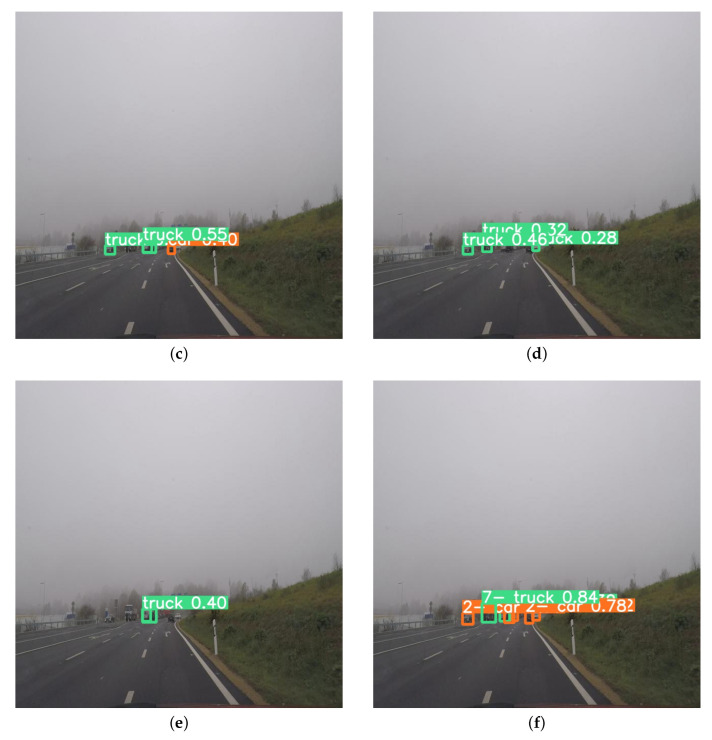
\includegraphics[width=.5\textwidth]{obj_det.jpg}
	\caption{Object Detection}
	\label{fig: img2}
\end{figure}

\subsection{Development of Machine Intelligence for Self-Driving Vehicles Through Video Capturing}
\begin{itemize}
    \item \textbf{Title:} Development of Machine Intelligence for Self-Driving Vehicles Through Video Capturing \cite{lowe2024development}
    \item \textbf{Authors:} Jordon Lowe and Kaya Kuru
    \item \textbf{Institution:} University of Central Lancashire, UK
    \item \textbf{Year:} 2024
    \item \textbf{Key Points:}
    \begin{itemize}
        \item The study explores the use of Deep Learning (DL) and Reinforcement Learning (RL) to enhance the intelligence of Self-Driving Vehicles (SDVs), aiming for Level 5 autonomy.
        \item Two systems were implemented:
        \begin{itemize}
            \item A CNN-based detector for traffic sign classification (93.78\% accuracy)
            \item A Faster R-CNN system for real-time object detection in videos, achieving high sensitivity and specificity
        \end{itemize}
        \item The Faster R-CNN integrates lane detection, vehicle tracking, and text-to-speech alerts, demonstrating practical applicability in autonomous driving.
        \item Challenges include dataset quality (e.g., false positives in CNN) and the need for DRL (Deep Reinforcement Learning) to handle dynamic urban environments.
    \end{itemize}
    \item \textbf{Contributions:}
    \begin{itemize}
        \item Framework for visual perception in SDVs
        \item Validation of DL for state and situation awareness (SSA)
        \item Emphasis on 5G-enabled swarm intelligence and sensor fusion for future AV development
    \end{itemize}
\end{itemize}

\subsection{Traditional and Deep Learning Approaches}
\begin{itemize}
    \item \textbf{Title:} Object Detection in Autonomous Vehicles under Adverse Weather: A Review of Traditional and Deep Learning Approaches \cite{tahir2024object}
    \item \textbf{Author:} Tahir, Noor Ul Ain and Zhang, Zuping and Asim, Muhammad and Chen, Junhong and ELAffendi, Mohammed
    \item \textbf{Journal:} Algorithms, MDPI
    \item \textbf{Year:} March 2024
    \item \textbf{Key Points:}
    \begin{itemize}
        \item Enhancing the environmental perception of autonomous vehicles (AVs) in intelligent transportation systems requires effective computer vision technology for object and obstacle detection.
        \item The study focuses on object detection under adverse weather conditions such as rain, fog, and snow.
        \item Traditional computer vision methods experience significant performance degradation when visual sensors are affected by harsh weather.
        \item Deep learning approaches provide improved robustness compared to traditional methods.
        \item However, deep learning methods still struggle to maintain consistent accuracy across a wide range of adverse weather scenarios.
    \end{itemize}
\end{itemize}

\subsection{Deep Learning-Based Detection Framework}
\begin{itemize}
    \item \textbf{Title:} Detection in Adverse Weather Conditions for Autonomous Vehicles via Deep Learning \cite{al2022detection}
    \item \textbf{Author:} Al-Haija, Qasem Abu and Gharaibeh, Manaf and Odeh, Ammar
    \item \textbf{Journal:} AI, MDPI
    \item \textbf{Year:} 2024
    \item \textbf{Key Points:}
    \begin{itemize}
        \item The paper proposes a deep learning (DL)-based detection framework to classify weather conditions encountered by autonomous vehicles.
        \item The framework utilizes transfer learning techniques and GPU acceleration to enhance weather classification accuracy.
        \item Integration of weather detection with object recognition enables context-aware perception for autonomous systems.
        \item Experimental results show improved object detection performance when weather conditions are automatically identified and system parameters are adapted in response.
    \end{itemize}
\end{itemize}

\subsection{Deep Learning-Based Robust Positioning}
\begin{itemize}
    \item \textbf{Title:} Deep learning-based robust positioning for all-weather autonomous driving \cite{almalioglu2022deep}
    \item \textbf{Author:} Almalioglu, Yasin and Turan, Mehmet and Trigoni, Niki and Markham, Andrew
    \item \textbf{Journal:} Nature Machine Intelligence
    \item \textbf{Year:} 2022
    \item \textbf{Key Points:}
    \begin{itemize}
        \item The paper proposes a deep learning-based self-supervised approach for ego-motion estimation, offering robust localization under inclement weather conditions.
        \item Geometry-aware methods are used to attentively fuse features, enhancing the positioning robustness.
        \item Self-supervised learning minimizes the need for labeled training data while maintaining performance.
        \item Integration with existing localization systems improves redundancy and reliability in autonomous vehicle navigation.
    \end{itemize}
\end{itemize}

\section{Multi-Objective Weather Classification and Object Detection}

\begin{figure}[h]
	\centering
	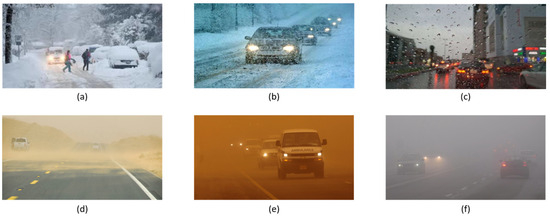
\includegraphics[width=.5\textwidth]{weather_condition_classification.jpg}
	\caption{Different Weather conditions}
	\label{fig: img2}
\end{figure}


\subsection{Integrated Weather Classification and Object Detection}
\begin{itemize}
    \item \textbf{Title:} Enhancing Autonomous Vehicle Perception in Adverse Weather: A Multi Objectives Model for Integrated Weather Classification and Object Detection \cite{aloufi2024enhancing}
    \item \textbf{Author:} Aloufi, Nasser and Alnori, Abdulaziz and Basuhail, Abdullah
    \item \textbf{Journal:} Electronics, MDPI
    \item \textbf{Year:} August 2024
    \item \textbf{Key Points:}
    \begin{itemize}
        \item Robust object detection and weather classification are critical for autonomous vehicle (AV) safety in adverse weather conditions.
        \item This paper introduces a multi-objective model that integrates weather classification and object detection tasks.
        \item The integrated framework improves computational efficiency and reduces latency by jointly processing both tasks.
        \item Joint optimization allows for better resource utilization and higher overall performance.
        \item Experimental results demonstrate improved accuracy compared to approaches that process weather and objects separately.
    \end{itemize}
\end{itemize}

\subsection{Data Merging and YOLOv8}
\begin{itemize}
    \item \textbf{Title:} Object Detection in Adverse Weather for Autonomous Driving through Data Merging and YOLOv8 \cite{kumar2023object}
    \item \textbf{Author:} Kumar, Debasis and Muhammad, Naveed
    \item \textbf{Journal:} PMC
    \item \textbf{Year:} October 2023
    \item \textbf{Key Points:}
    \begin{itemize}
        \item Perception is a key component in autonomous driving for understanding the environment through sensors.
        \item This study applies the YOLOv8 architecture tailored for adverse weather detection.
        \item Data merging integrates multiple sensor inputs to enhance detection reliability in rain, fog, and low-light conditions.
        \item The results show a significant improvement in object detection accuracy under challenging scenarios.
    \end{itemize}
\end{itemize}

\section{Lane Detection Using Deep Learning}


\begin{figure}[h]
	\centering
	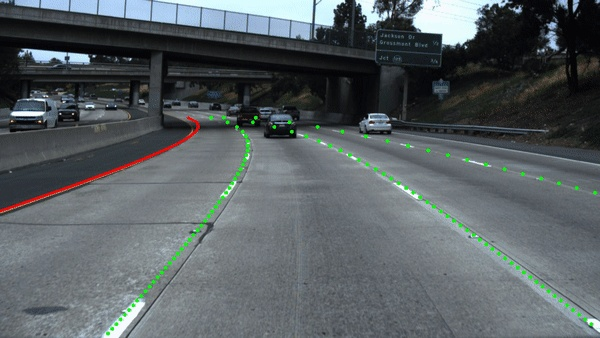
\includegraphics[width=.5\textwidth]{Lane_Detection_Demo.jpg}
	\caption{Lane Detection}
	\label{fig: img2}
\end{figure}

\subsection{Semantic Segmentation and Edge Detection}
\begin{itemize}
    \item \textbf{Title:} Improved Lane Detection for Autonomous Vehicles Using Deep Learning, Semantic Segmentation, Edge Detection and Multi-Sensor Data Fusion \cite{ali2024improved}
    \item \textbf{Author:} Ali, Babar and Akbar, Muhammad Mohsin and Baqir, Muhammad Uzair and Sajid, Muhammad Umair and Soomro, Abdul Majid and Sikander, Ammar and Rehman, Attique Ur and Khurshid, Imran
    \item \textbf{Journal:} South Florida Journal of Development
    \item \textbf{Year:} 2024
    \item \textbf{Key Points:}
    \begin{itemize}
        \item Combines semantic segmentation and edge detection for enhanced lane detection accuracy.
        \item Achieves lane detection accuracy of 97.8\%, specificity of 99.28\%, and average processing time of 0.0047 seconds per epoch.
        \item Multi-sensor fusion with data from cameras and LiDAR improves robustness and accuracy.
        \item Capable of real-time lane detection suitable for AV deployment.
    \end{itemize}
\end{itemize}

\subsection{Optimizing Lane Detection and Steering}
\begin{itemize}
    \item \textbf{Title:} A Framework for Optimizing Deep Learning-Based Lane Detection and Steering for Autonomous Driving \cite{yordanov2024framework}
    \item \textbf{Author:} Yordanov, Daniel and Chakraborty, Ashim and Hasan, Md Mahmudul and Cirstea, Silvia
    \item \textbf{Journal:} PMC
    \item \textbf{Year:} December 2024
    \item \textbf{Key Points:}
    \begin{itemize}
        \item Proposes an end-to-end framework combining lane detection with vehicle steering control.
        \item Virtual sandbox environment in Unity3D supports procedural road and driving scenario generation.
        \item Enables systematic testing under a variety of road and environmental conditions.
        \item Enhances real-time responsiveness and adaptability of self-driving systems.
    \end{itemize}
\end{itemize}

\subsection{Lane Following Network}
\begin{itemize}
    \item \textbf{Title:} Deep-Learning-Based Network for Lane Following in Autonomous Vehicles \cite{khanum2022deep}
    \item \textbf{Author:} Khanum, Abida and Lee, Chao-Yang and Yang, Chu-Sing
    \item \textbf{Journal:} Electronics, MDPI
    \item \textbf{Year:} September 2022
    \item \textbf{Key Points:}
    \begin{itemize}
        \item Introduces a VGG16 and GRU-based deep learning architecture for lane following.
        \item GRU enables temporal consistency for smoother lane tracking across video frames.
        \item The network is effective in managing dynamic road changes and temporary occlusions.
        \item Demonstrates improved tracking and motion planning in varied road environments.
    \end{itemize}
\end{itemize}

\section{Research Gaps and Future Opportunities}

The reviewed literature reveals several critical areas requiring continued research and development:

\begin{itemize}
    \item \textbf{Limited Real-World Validation:} 
    While many studies demonstrate promising results in controlled environments, comprehensive validation under genuine adverse weather conditions remains limited. Most research relies on synthetic data augmentation or small-scale real-world datasets.
    
    \item \textbf{Computational Efficiency vs. Accuracy Trade-offs:} 
    Advanced deep learning models that achieve high accuracy often require substantial computational resources. This creates challenges for real-time deployment on automotive-grade embedded platforms with limited processing capabilities.
    
    \item \textbf{Generalization Across Geographic Regions:} 
    Models trained on specific datasets frequently struggle to generalize across different geographic regions. Variations in road infrastructure, weather patterns, and traffic dynamics necessitate extensive retraining to ensure robust performance.
    
    \item \textbf{Integration and System-Level Validation:} 
    There is limited research on integrating weather-adaptive perception systems into full autonomous vehicle control stacks. Furthermore, system-level validation encompassing perception, planning, and control under dynamic weather conditions is still lacking.
\end{itemize}

